\documentclass[12pt,xcolor=dvipsnames]{beamer}
\usepackage{soul}
\usepackage{xcolor}
\usepackage{subcaption}
\usepackage{outlines}
\usepackage{amsmath}
\usepackage{pgffor}
\usepackage{pgfplots}
\usepackage{etoolbox}
\usepackage{animate}
\usepackage{tcolorbox}
\usepackage{pgfgantt}
\usetheme{Copenhagen}

\definecolor{ImperialBlue}{RGB}{0,0,203} % UBC Blue (primary)
\definecolor{ImperialTeal}{RGB}{1, 255, 125} % UBC Blue (primary)
\setbeamercolor{title}{fg=ImperialTeal} % Set foreground color of title to blue
\setbeamercolor{frametitle}{fg=ImperialTeal} % Set foreground color of title to blue
\setbeamercolor{section in head/foot}{bg=ImperialTeal} % Set foreground color of block titles to green
\setbeamercolor{structure}{fg=ImperialBlue} % Set foreground color of block titles to green

\usepackage{tikz}
\usetikzlibrary{overlay-beamer-styles}

% Hide beamer nav. symbols
\setbeamertemplate{navigation symbols}{}

% To see ahead of presentation
% \setbeamercovered{transparent}
\setbeamertemplate{caption}{\raggedright\insertcaption\par}

% \usepackage{setspace}
% \onehalfspacing
\usepackage{graphicx}

% Code specific
\usepackage{listings}
\usepackage{xcolor}
\lstset{
keywordstyle=\color{blue}\bfseries,    % Keywords (e.g., if, for, class) will be blue and bold
commentstyle=\color{green!60!black}\em, % Comments will be a dark green and italicized
stringstyle=\color{red!90!black},      % Strings (text in quotes) will be dark red
language=C++, % Set default language to C++
basicstyle=\scriptsize\ttfamily, % Basic font settings
numbers=left, % Line numbers on the left
numberstyle=\tiny\color{gray}, % Style of the line numbers
frame=single, % Add a frame around the code
breaklines=true, % Automatic line breaking
backgroundcolor=\color{black!5}, % Light gray background
captionpos=b, % Caption position at the bottom
}

\title{Compressible flow}
\date{$15^{th}$ Dec 2025}

\begin{document}
\maketitle

\begin{frame}{Artifical Viscosity}
    Consider a conversative law with artifical viscosity of the form
    \begin{equation}
        \frac{\partial \mathbf{u}}{\partial t} + \nabla \cdot \mathbf{F} = \nabla(\epsilon \nabla \mathbf{u}) 
    \end{equation}
    where $\epsilon$ refers to the artifical viscosity,
    \begin{equation}
        \epsilon = \epsilon_0\frac{h}{p}\lambda_{max}S
    \end{equation}
    \begin{subequations}
    with $\lambda$ as the maximum characteristic speed and $S$ as the shock sensor,
    \begin{equation}
        S = log_{10} \frac{\langle u - \tilde{u}, u - \tilde{u} \rangle }{\langle u, u \rangle}
    \end{equation}
    \begin{equation}
        u = \sum^P_i \hat{u}_i \phi_i, \quad \tilde{u} = \sum^{P-1}_i \hat{u}_i \phi_i
    \end{equation}
    
    
    \end{subequations}
\end{frame}

\begin{frame}{Sod's Shock Tube, $N_{el} = 4, \epsilon_0 = 1$}
    \begin{figure}
    \centering
    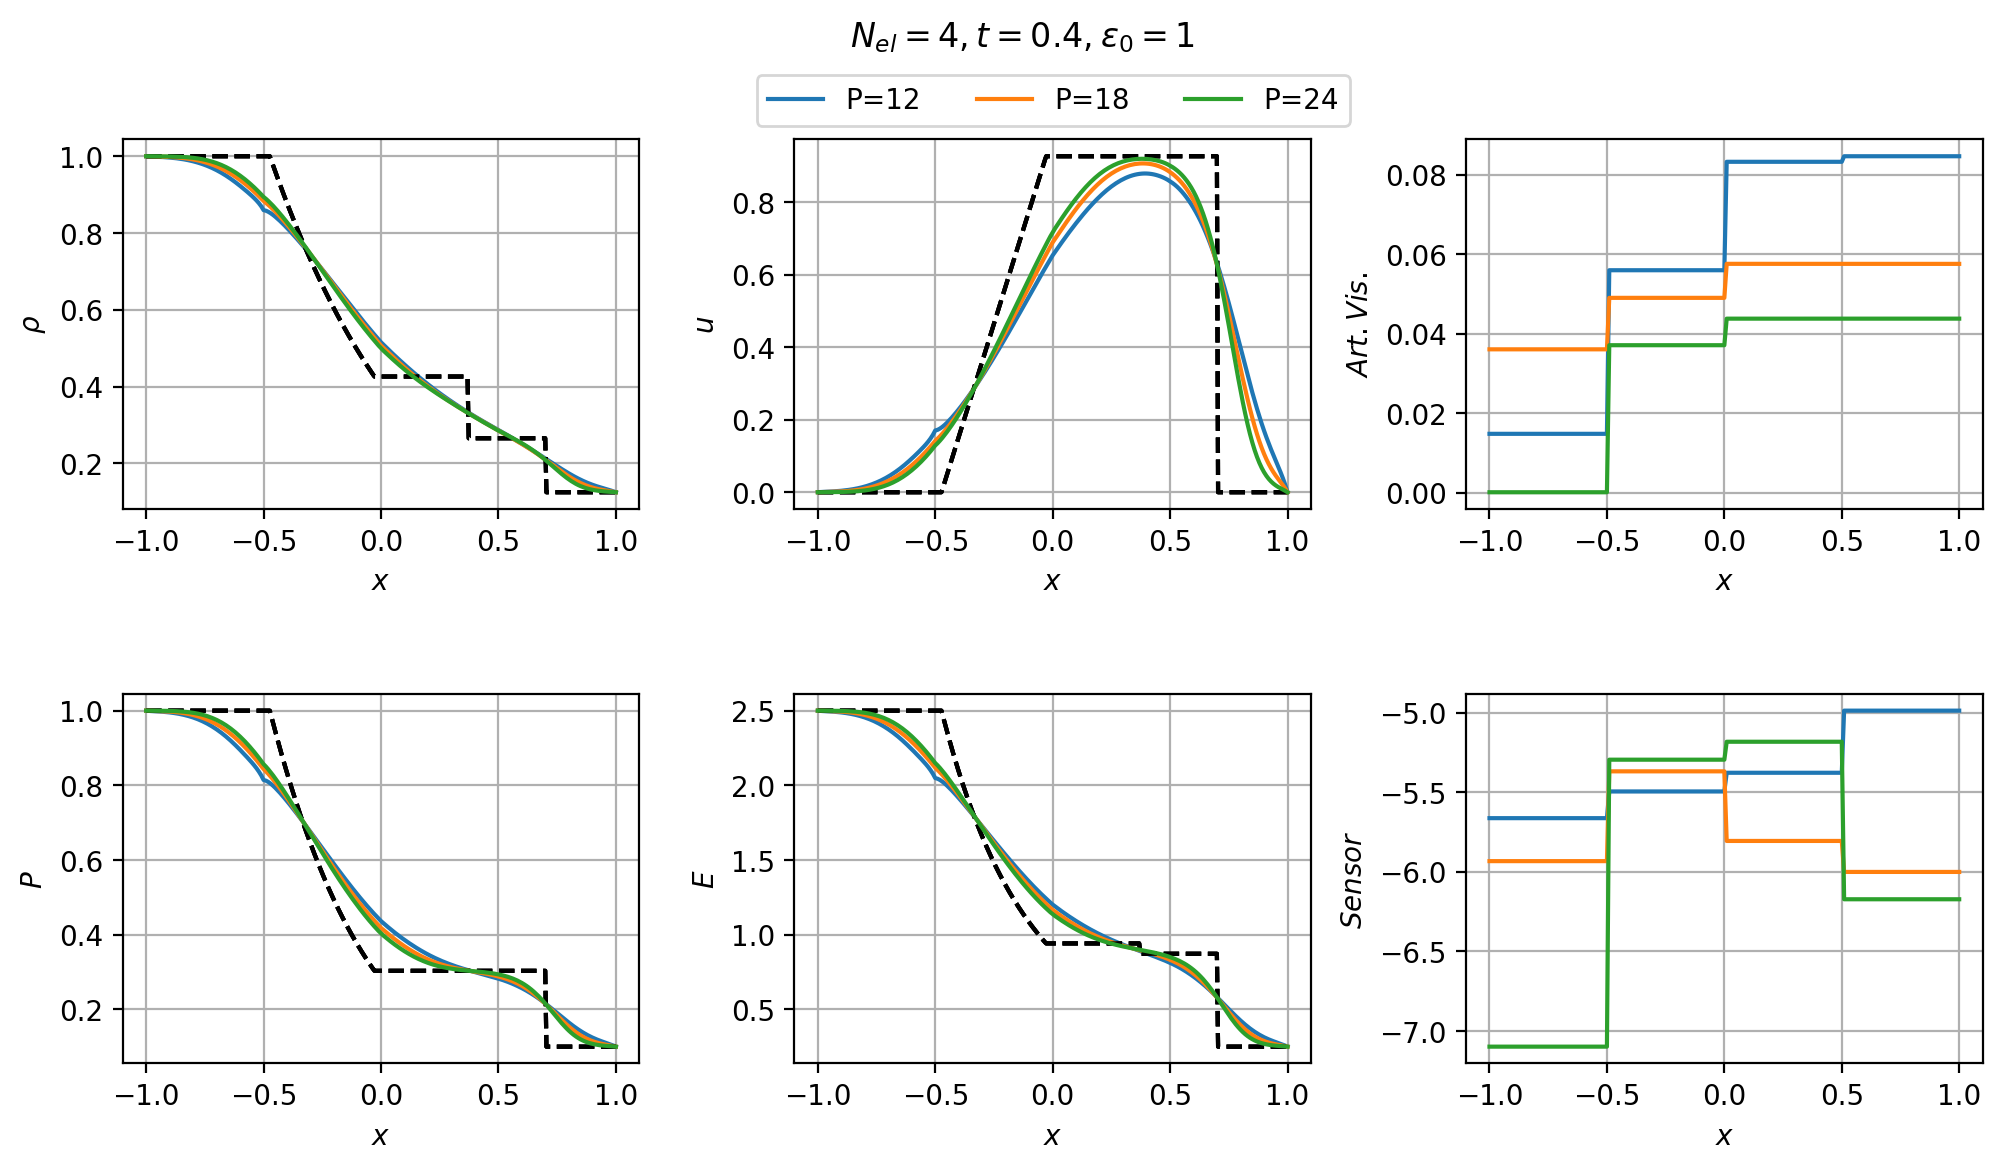
\includegraphics[width=\textwidth]{../SodTube/Nel4/plot_4.png}
    \end{figure}
\end{frame}

\begin{frame}{Sod's Shock Tube, $N_{el} = 4, \epsilon_0 = 0.1$}
    \begin{figure}
    \centering
    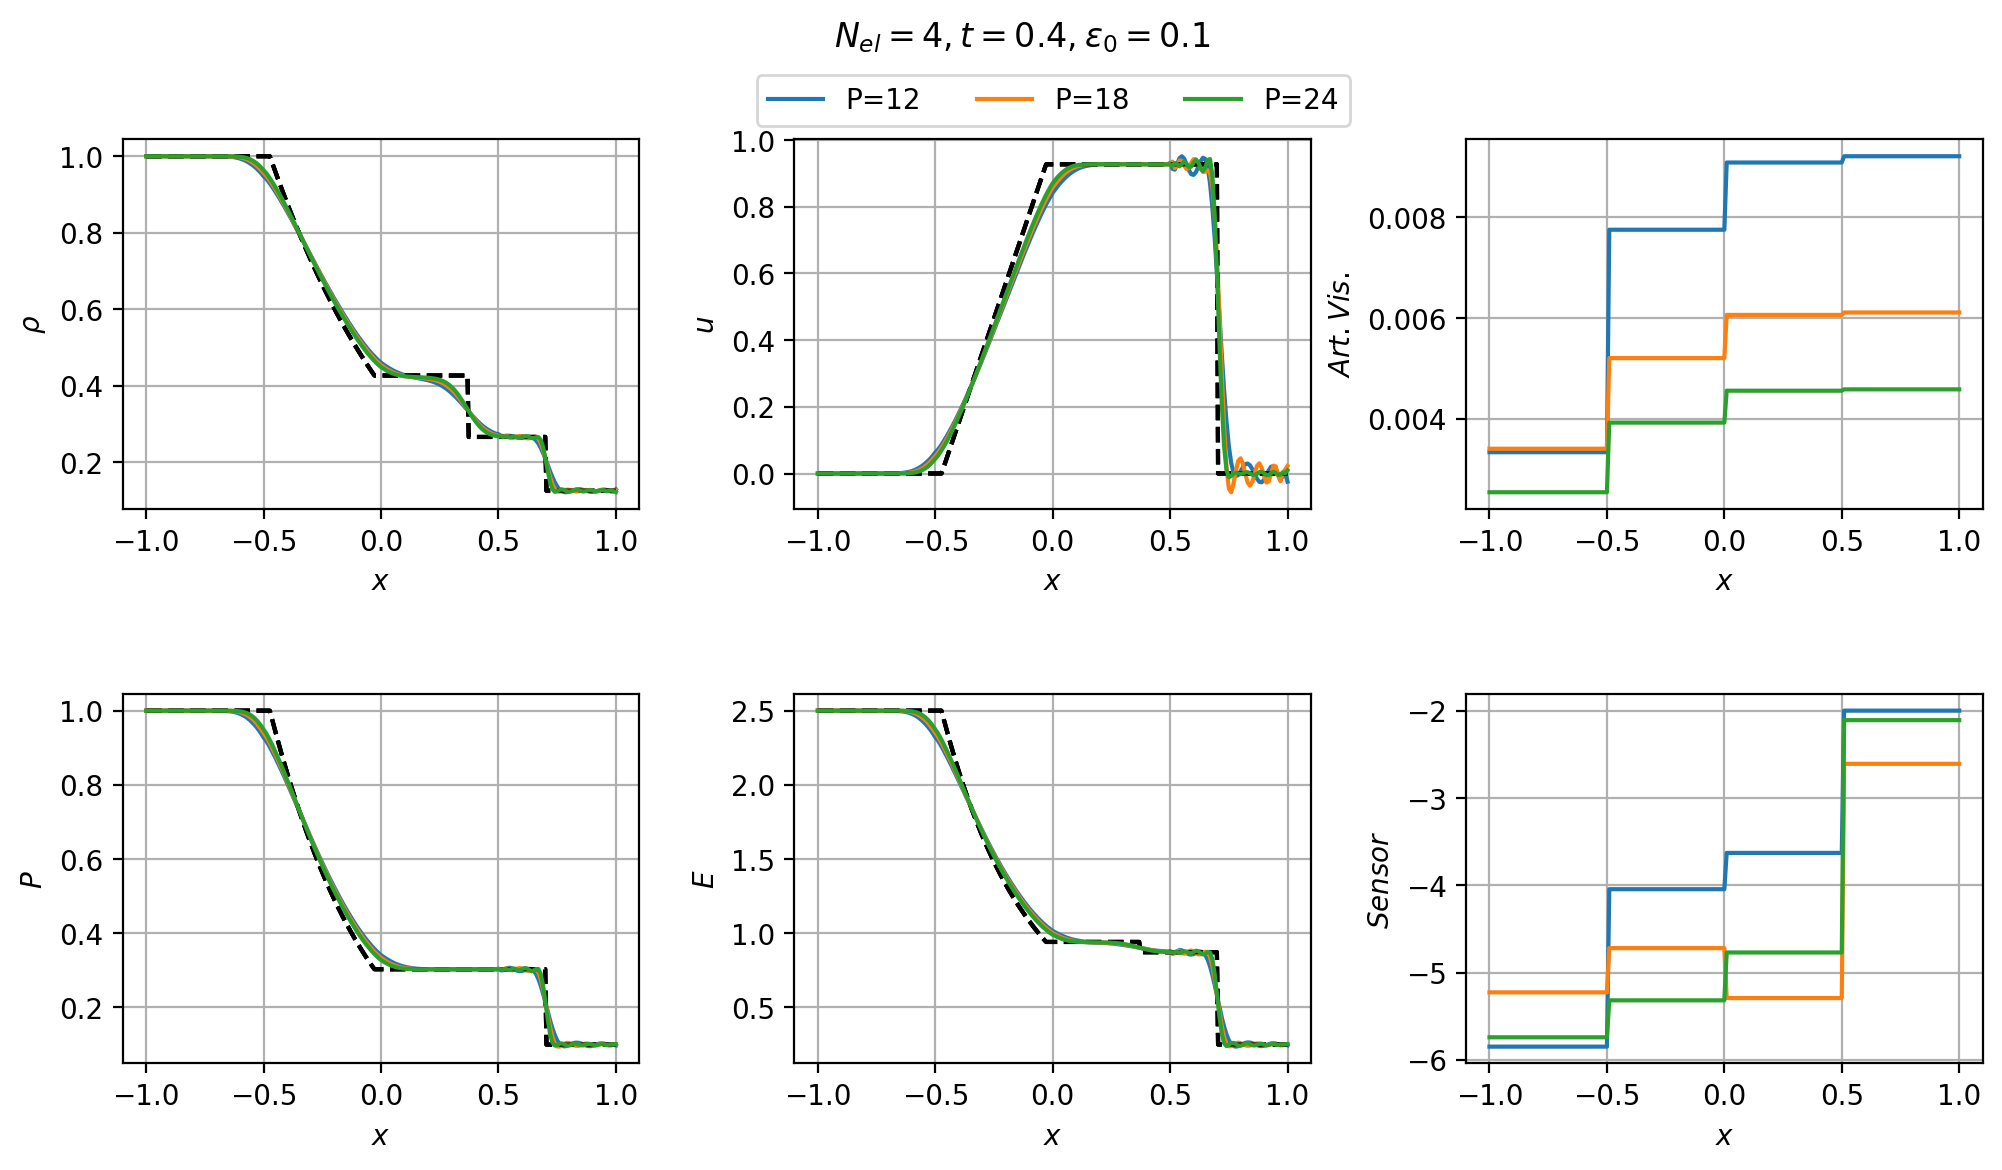
\includegraphics[width=\textwidth]{../SodTube/Nel4-mu0.1/plot_4.png}
    \end{figure}
\end{frame}

\begin{frame}{Sod's Shock Tube, $N_{el} = 16, \epsilon_0 = 0.1$}
    \begin{figure}
    \centering
    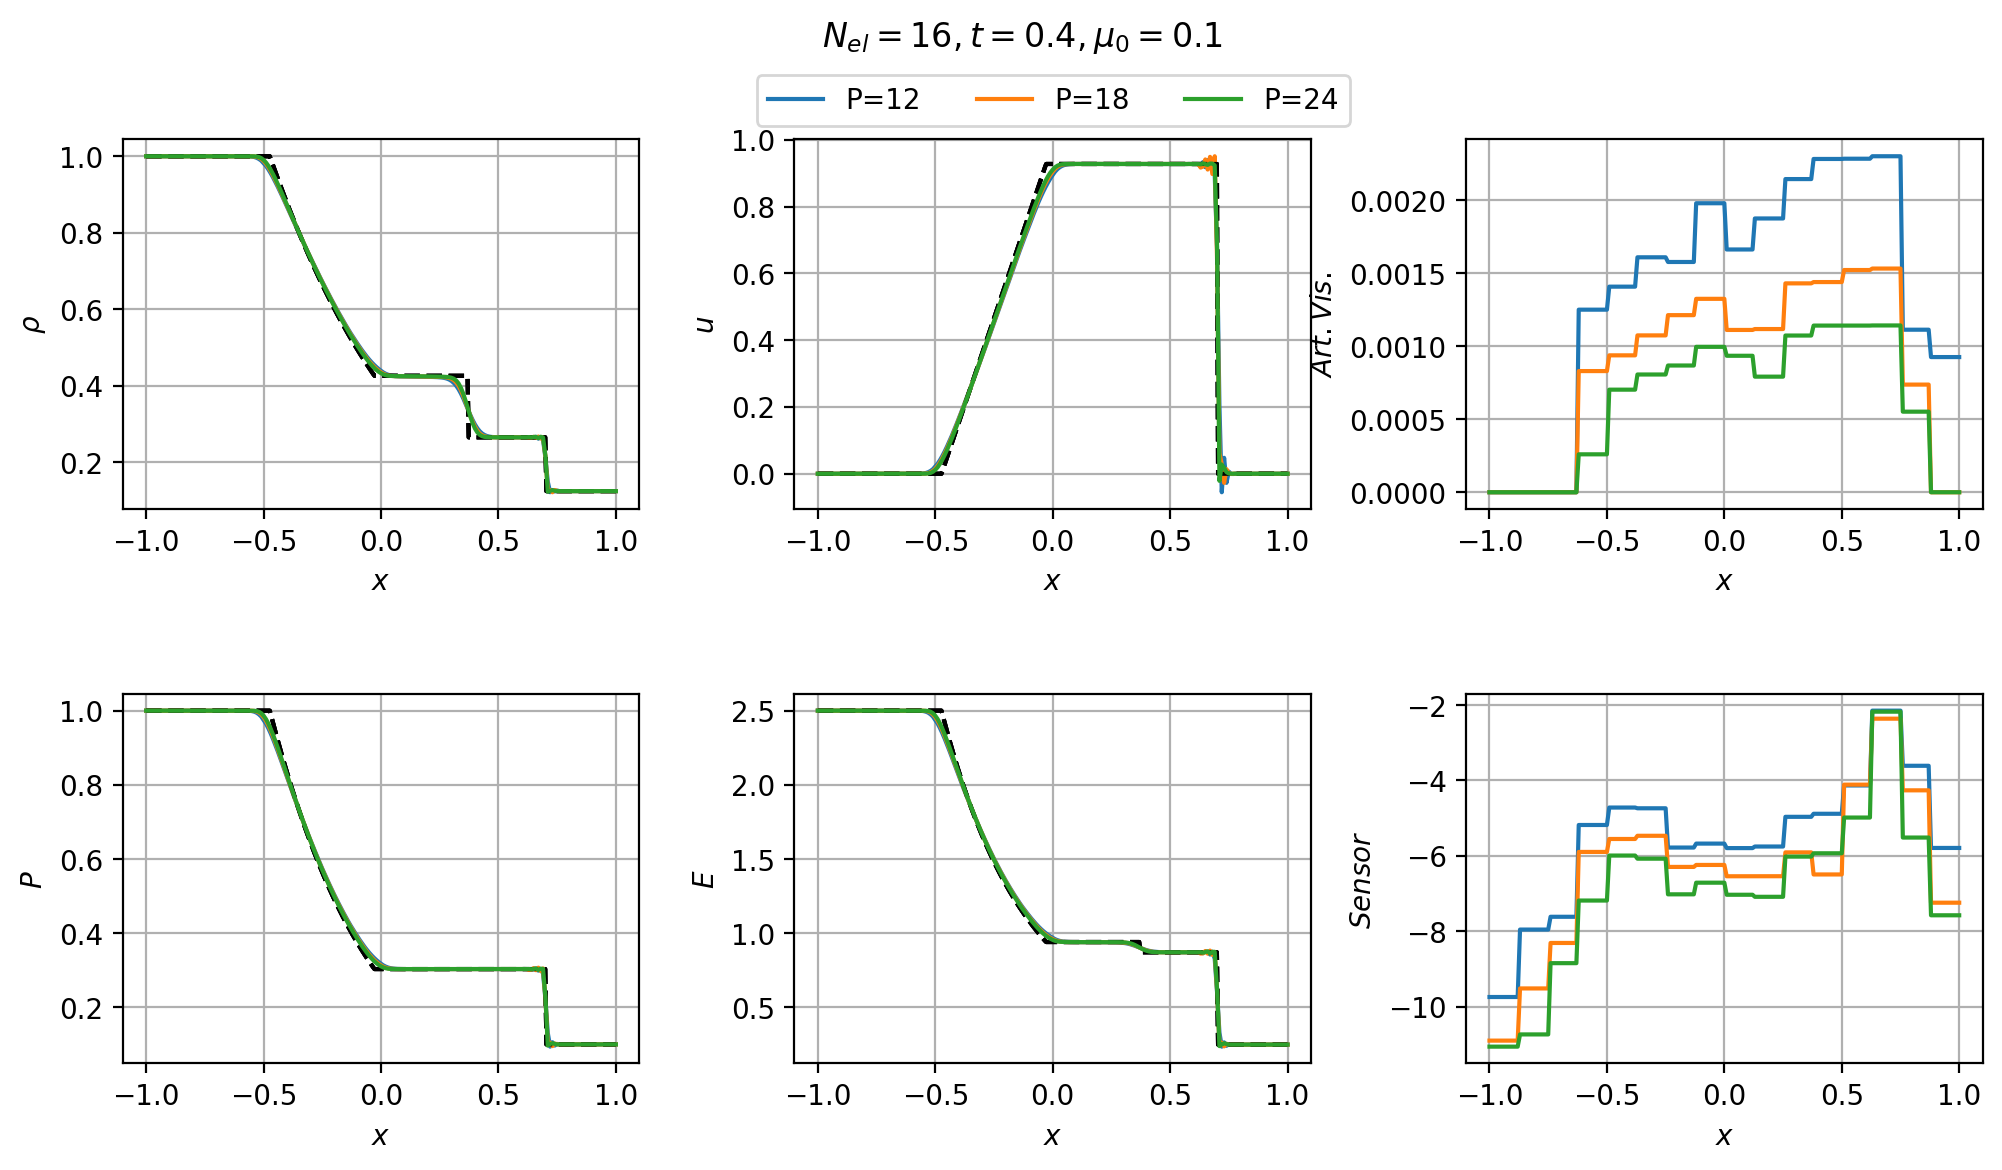
\includegraphics[width=\textwidth]{../SodTube/Nel16-mu0.1/plot_4.png}
    \end{figure}
\end{frame}

\begin{frame}{Leblanc's Shock Tube, $N_{el} = 200, t=0, \epsilon_0 = 1$}
    \begin{figure}
    \centering
    
\includegraphics[width=\textwidth]{plot_0.png}
    \end{figure}
\end{frame}

\begin{frame}{Leblanc's Shock Tube, $N_{el} = 200, t=1, \epsilon_0 = 1$}
    \begin{figure}
    \centering
    
\includegraphics[width=\textwidth]{plot_1.png}
    \end{figure}
\end{frame}

\begin{frame}{Leblanc's Shock Tube, $N_{el} = 200, t=2, \epsilon_0 = 1$}
    \begin{figure}
    \centering
    
\includegraphics[width=\textwidth]{plot_2.png}
    \end{figure}
\end{frame}

\begin{frame}{Leblanc's Shock Tube, $N_{el} = 200, t=3, \epsilon_0 = 1$}
    \begin{figure}
    \centering
    
\includegraphics[width=\textwidth]{plot_3.png}
    \end{figure}
\end{frame}


\end{document}

